\documentclass[12pt]{article}

\usepackage{amsmath}
\usepackage{amssymb}
\usepackage{graphicx}
\usepackage{caption}

\title{Further Functions (Assessment)}
\author{Zac Hart}

\graphicspath{{./graphs/}}

\DeclareCaptionLabelFormat{custom}{Fig. #2}
\captionsetup{format=hang, labelformat=custom, labelsep=period, labelfont=bf}

\begin{document}

\maketitle

\section*{Answers}

\begin{enumerate}

    % 1.
    \item The chosen function is $f(x)=\ln{x}$. (Fig. \ref{fig:graph-1})

        \begin{enumerate}

            % 1.a.
            \item $|y|=f(x)$ is the reflection of $y=f(x)$ about the $x$-axis, and is undefined for negative $y$.

            % 1.b.
            \item To sketch the graph of $|y|=f(x)$ for any functon, first sketch the graph of $y=f(x)$ for all positive values of $y$. Then sketch the reflection of this function about the $x$-axis.

            \begin{figure}[h]
                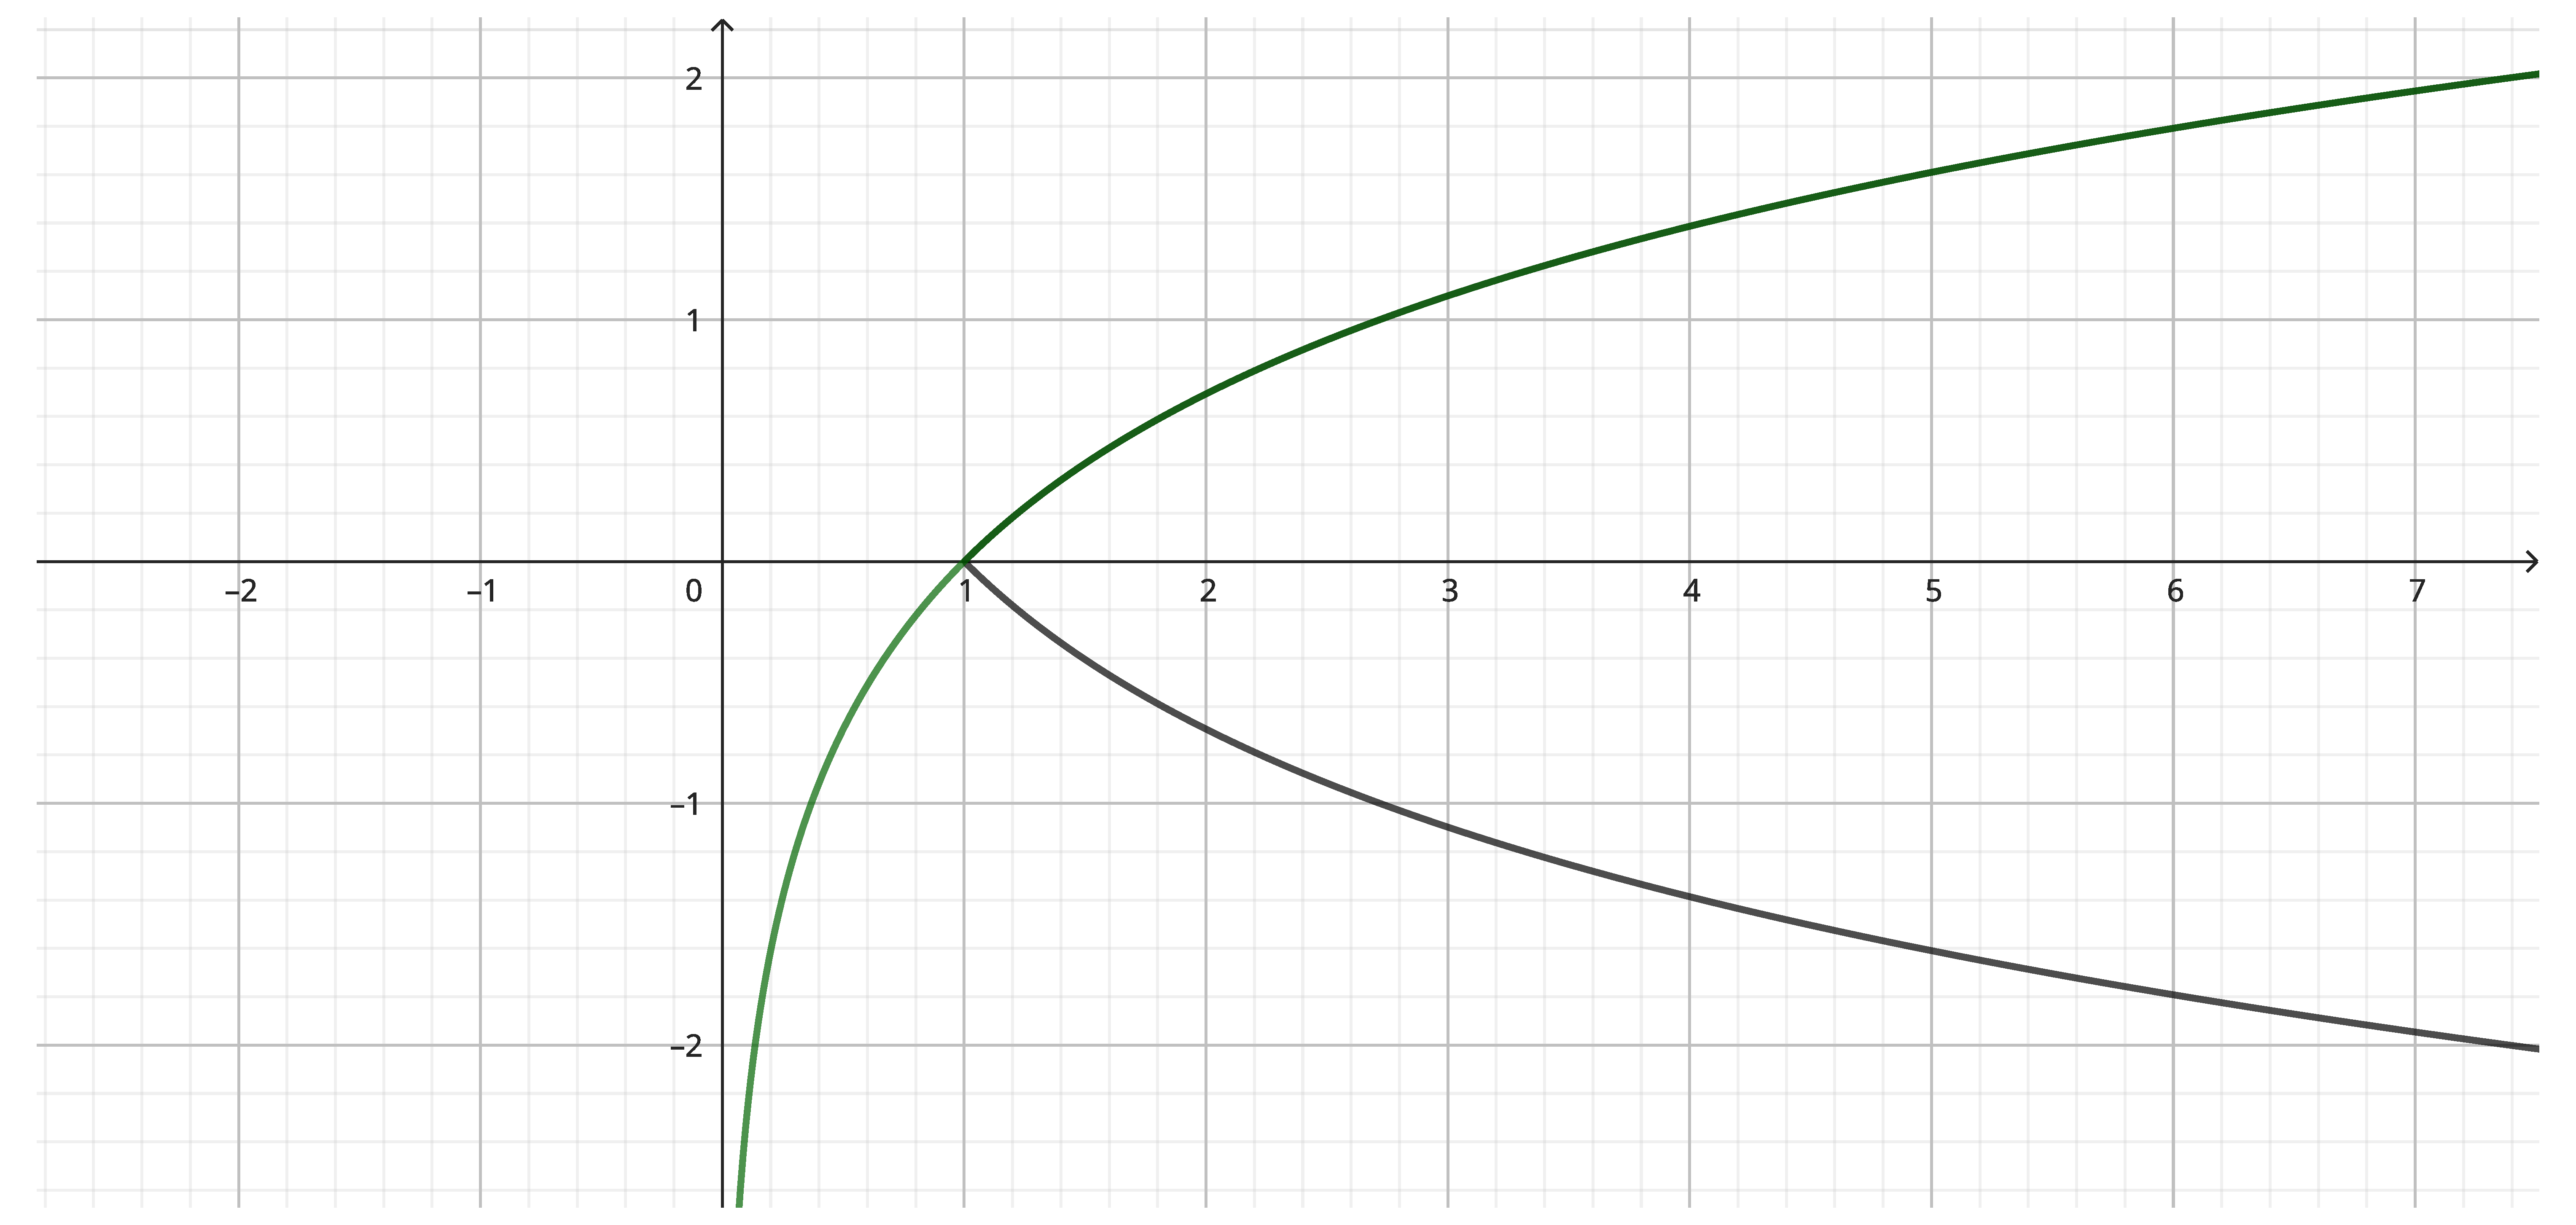
\includegraphics[width=\textwidth]{graph-1.pdf}
                \caption{$y=f(x)$ (green) and $|y|=f(x)$ (black).}
                \label{fig:graph-1}
            \end{figure}

            % 1.c.
            \item Steve is partially correct because his interpretation of $|y|=f(x)$ includes the values of $f(x)$ and its reflection about the $x$-axis, however he neglects the fact that $|y|\ne f(x)$ when $y$ is negative.\\Suppose that $\Phi(x)=\frac{1}{x}$. When x is negative, $\Phi(x)$ is also negative. Therefore the function $|y|=\Phi(x)$ is undefined for negative $x$: $|y|$ is positive and $\Phi(x)$ is negative, hence they are not equal.\\For positive values of $x$, however, the equation is satisfied.

            % 1.d.
            \item $f(x)=-x^2-1$ is negative for all $x$, so $|y|=f(x)$ is undefined for all $x$. (Fig. \ref{fig:graph-2})\\$g(x)=x^2+1$ is positive for all $x$, so $|y|=g(x)$ is identical to $y=g(x)$. (Fig. \ref{fig:graph-2})

        \end{enumerate}

        \begin{figure}[h]
            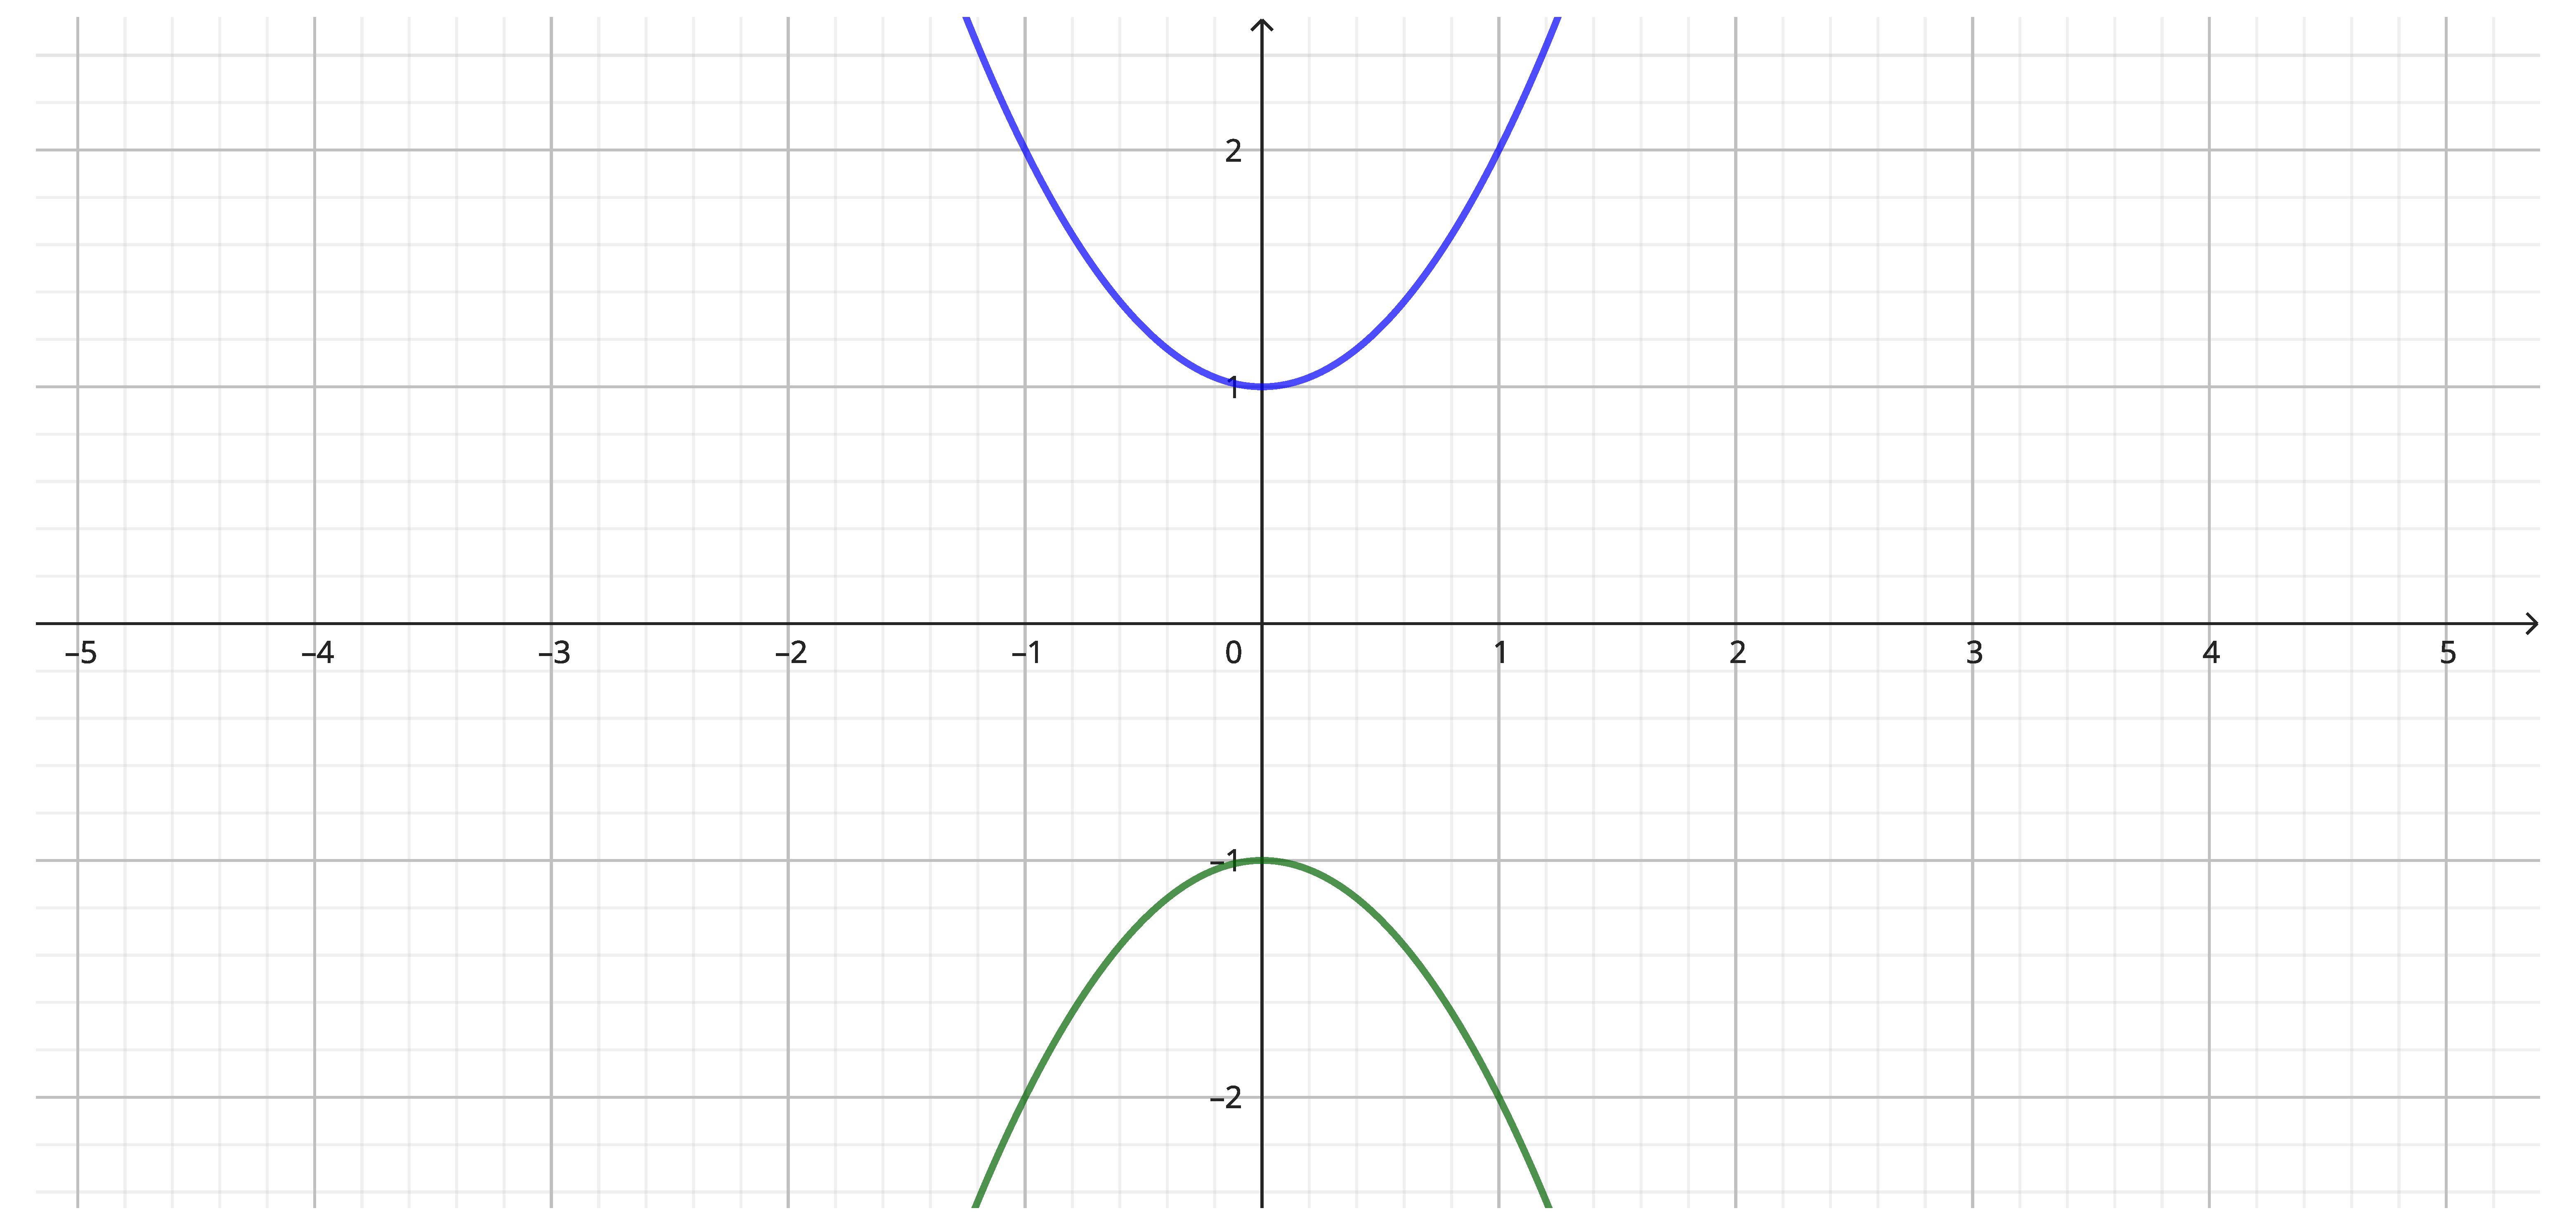
\includegraphics[width=\textwidth]{graph-2.pdf}
            \caption{$y=f(x)$ (green) and $y=g(x)$ (blue).}
            \label{fig:graph-2}
        \end{figure}


    % 2.
    \item The chosen function is $f(x)=x^3$. (Fig. \ref{fig:graph-3})

    \begin{enumerate}

        %2.a.
        \item $y=f(4-x^3)$ is the reflection of $y=f(x)$ about the $y$-axis, translated right by 4 units. (Fig. \ref{fig:graph-3})

        %2.b.
        \item To sketch $f(a-x)$ for any function, first sketch $y=f(-x)$, which is $y=f(x)$ reflected about the $y$-axis. Then sketch $y=f(-x)$ translated right by $a$.

        %2.c.
        \item Since $f(a-x)=f(-(x-a))$, $f(a-x)$ is the reflection of $f(x-a)$ about the $y$-axis. This transformation of $f(x)$ has the same effect as reflecting the function about the $y$-axis first then translating it right by $a$.

        \begin{figure}[h]
            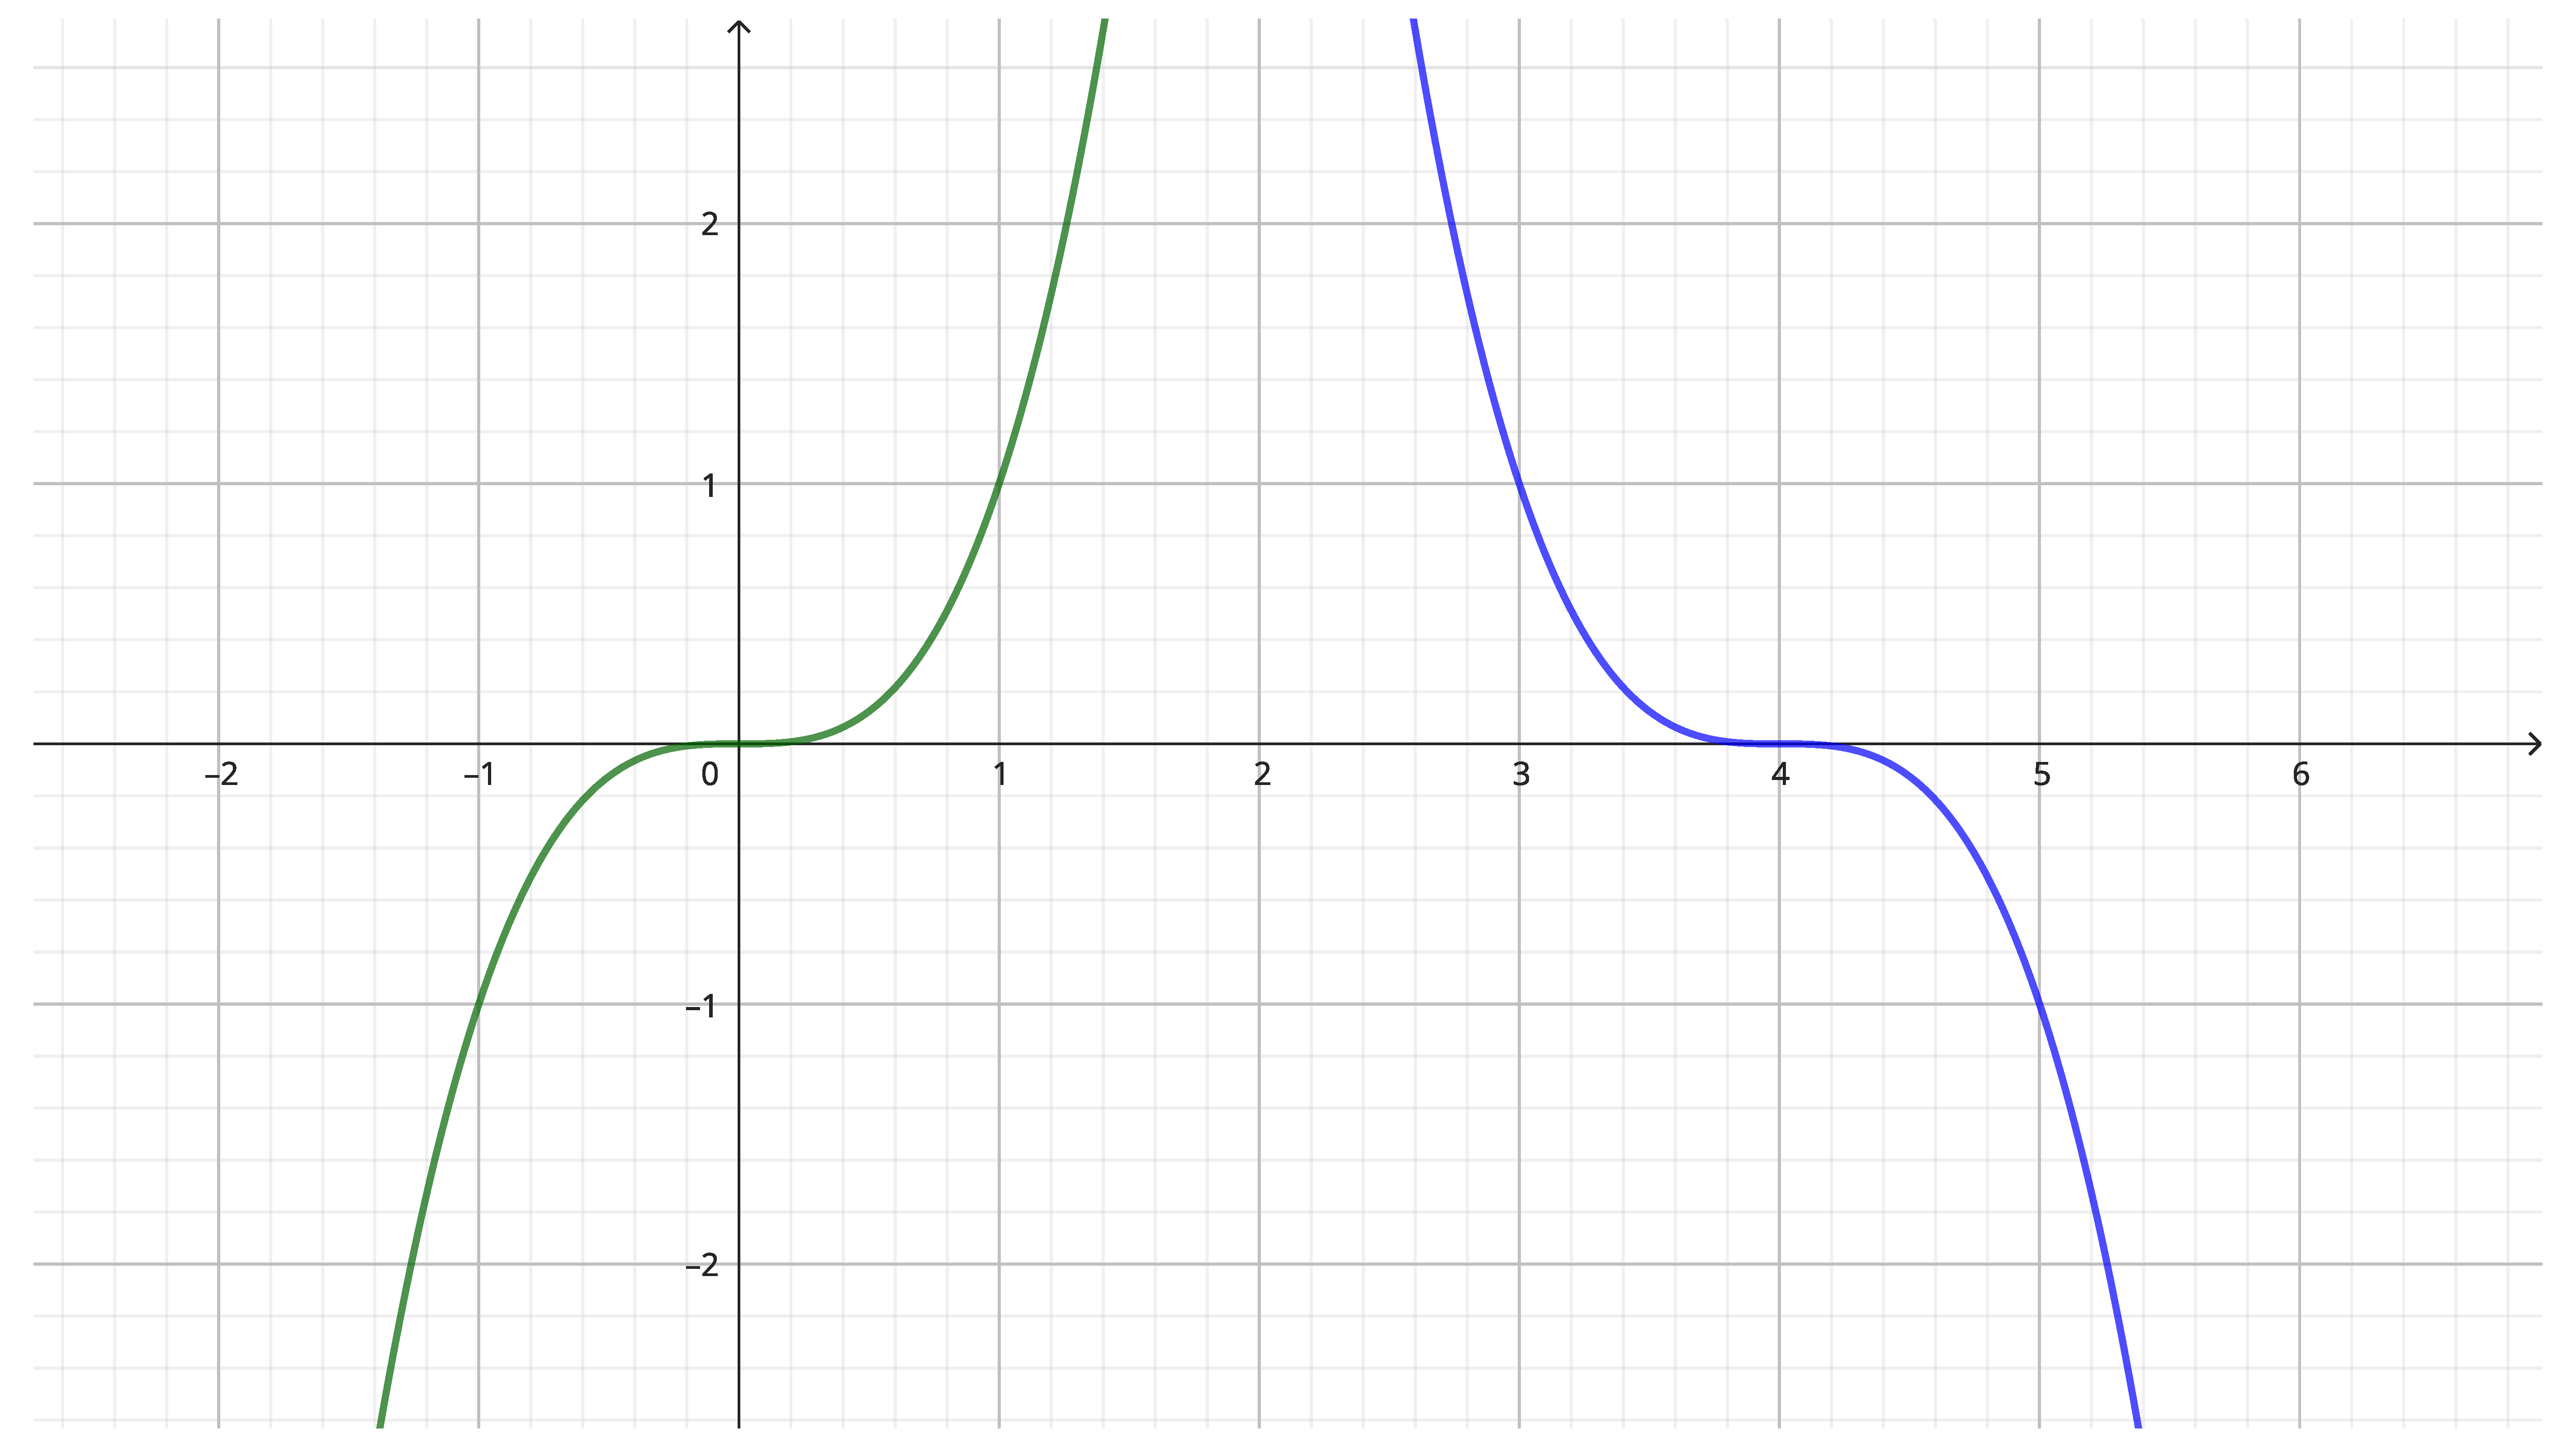
\includegraphics[width=\textwidth]{graph-3.pdf}
            \caption{$y=f(x)$ (green) and $y=f(4-x)$ (blue).}
            \label{fig:graph-3}
        \end{figure}

    \end{enumerate}

    % 3.
    \item \begin{enumerate}

        % 3.a.
        \item \begin{flalign*}
            \intertext{We are given that}
            &&xy-x-2y-2&=0&\\
            \text{so}&&xy-x-2y+2&=4&\\
            \text{and}&&(x-2)(y-1)&=4& \tag{1} \label{eq:1}
        \end{flalign*}

        \begin{enumerate}

            % 3.a.i.
            \item We choose the new set of axis as
            \begin{equation*}
                X=x+2\quad Y=y+1
            \end{equation*}

            % 3.a.ii.
            \item \begin{gather*}
                \intertext{From \eqref{eq:1} we get}
                XY=4
                \intertext{therefore the tranformed function is}
                XY-4=0
            \end{gather*}

            % 3.a.iii.
            \item The asymptotes of the hyperbola with respect to the original set of axis are $x=2$, $y=1$.

            % 3.a.iv.
            \item The asymptotes of the hyperbola with respect to the new set of axis are $x=0$, $y=0$.

        \end{enumerate}

        % 3.b.
        \item \begin{gather}
            \label{eq:2}
            xy=1\\
            \label{eq:3}
            \begin{aligned}
                X&=x\cos\theta-y\sin\theta\\
                Y&=x\sin\theta+y\cos\theta
            \end{aligned}
        \end{gather}
        \begin{figure}[h]
            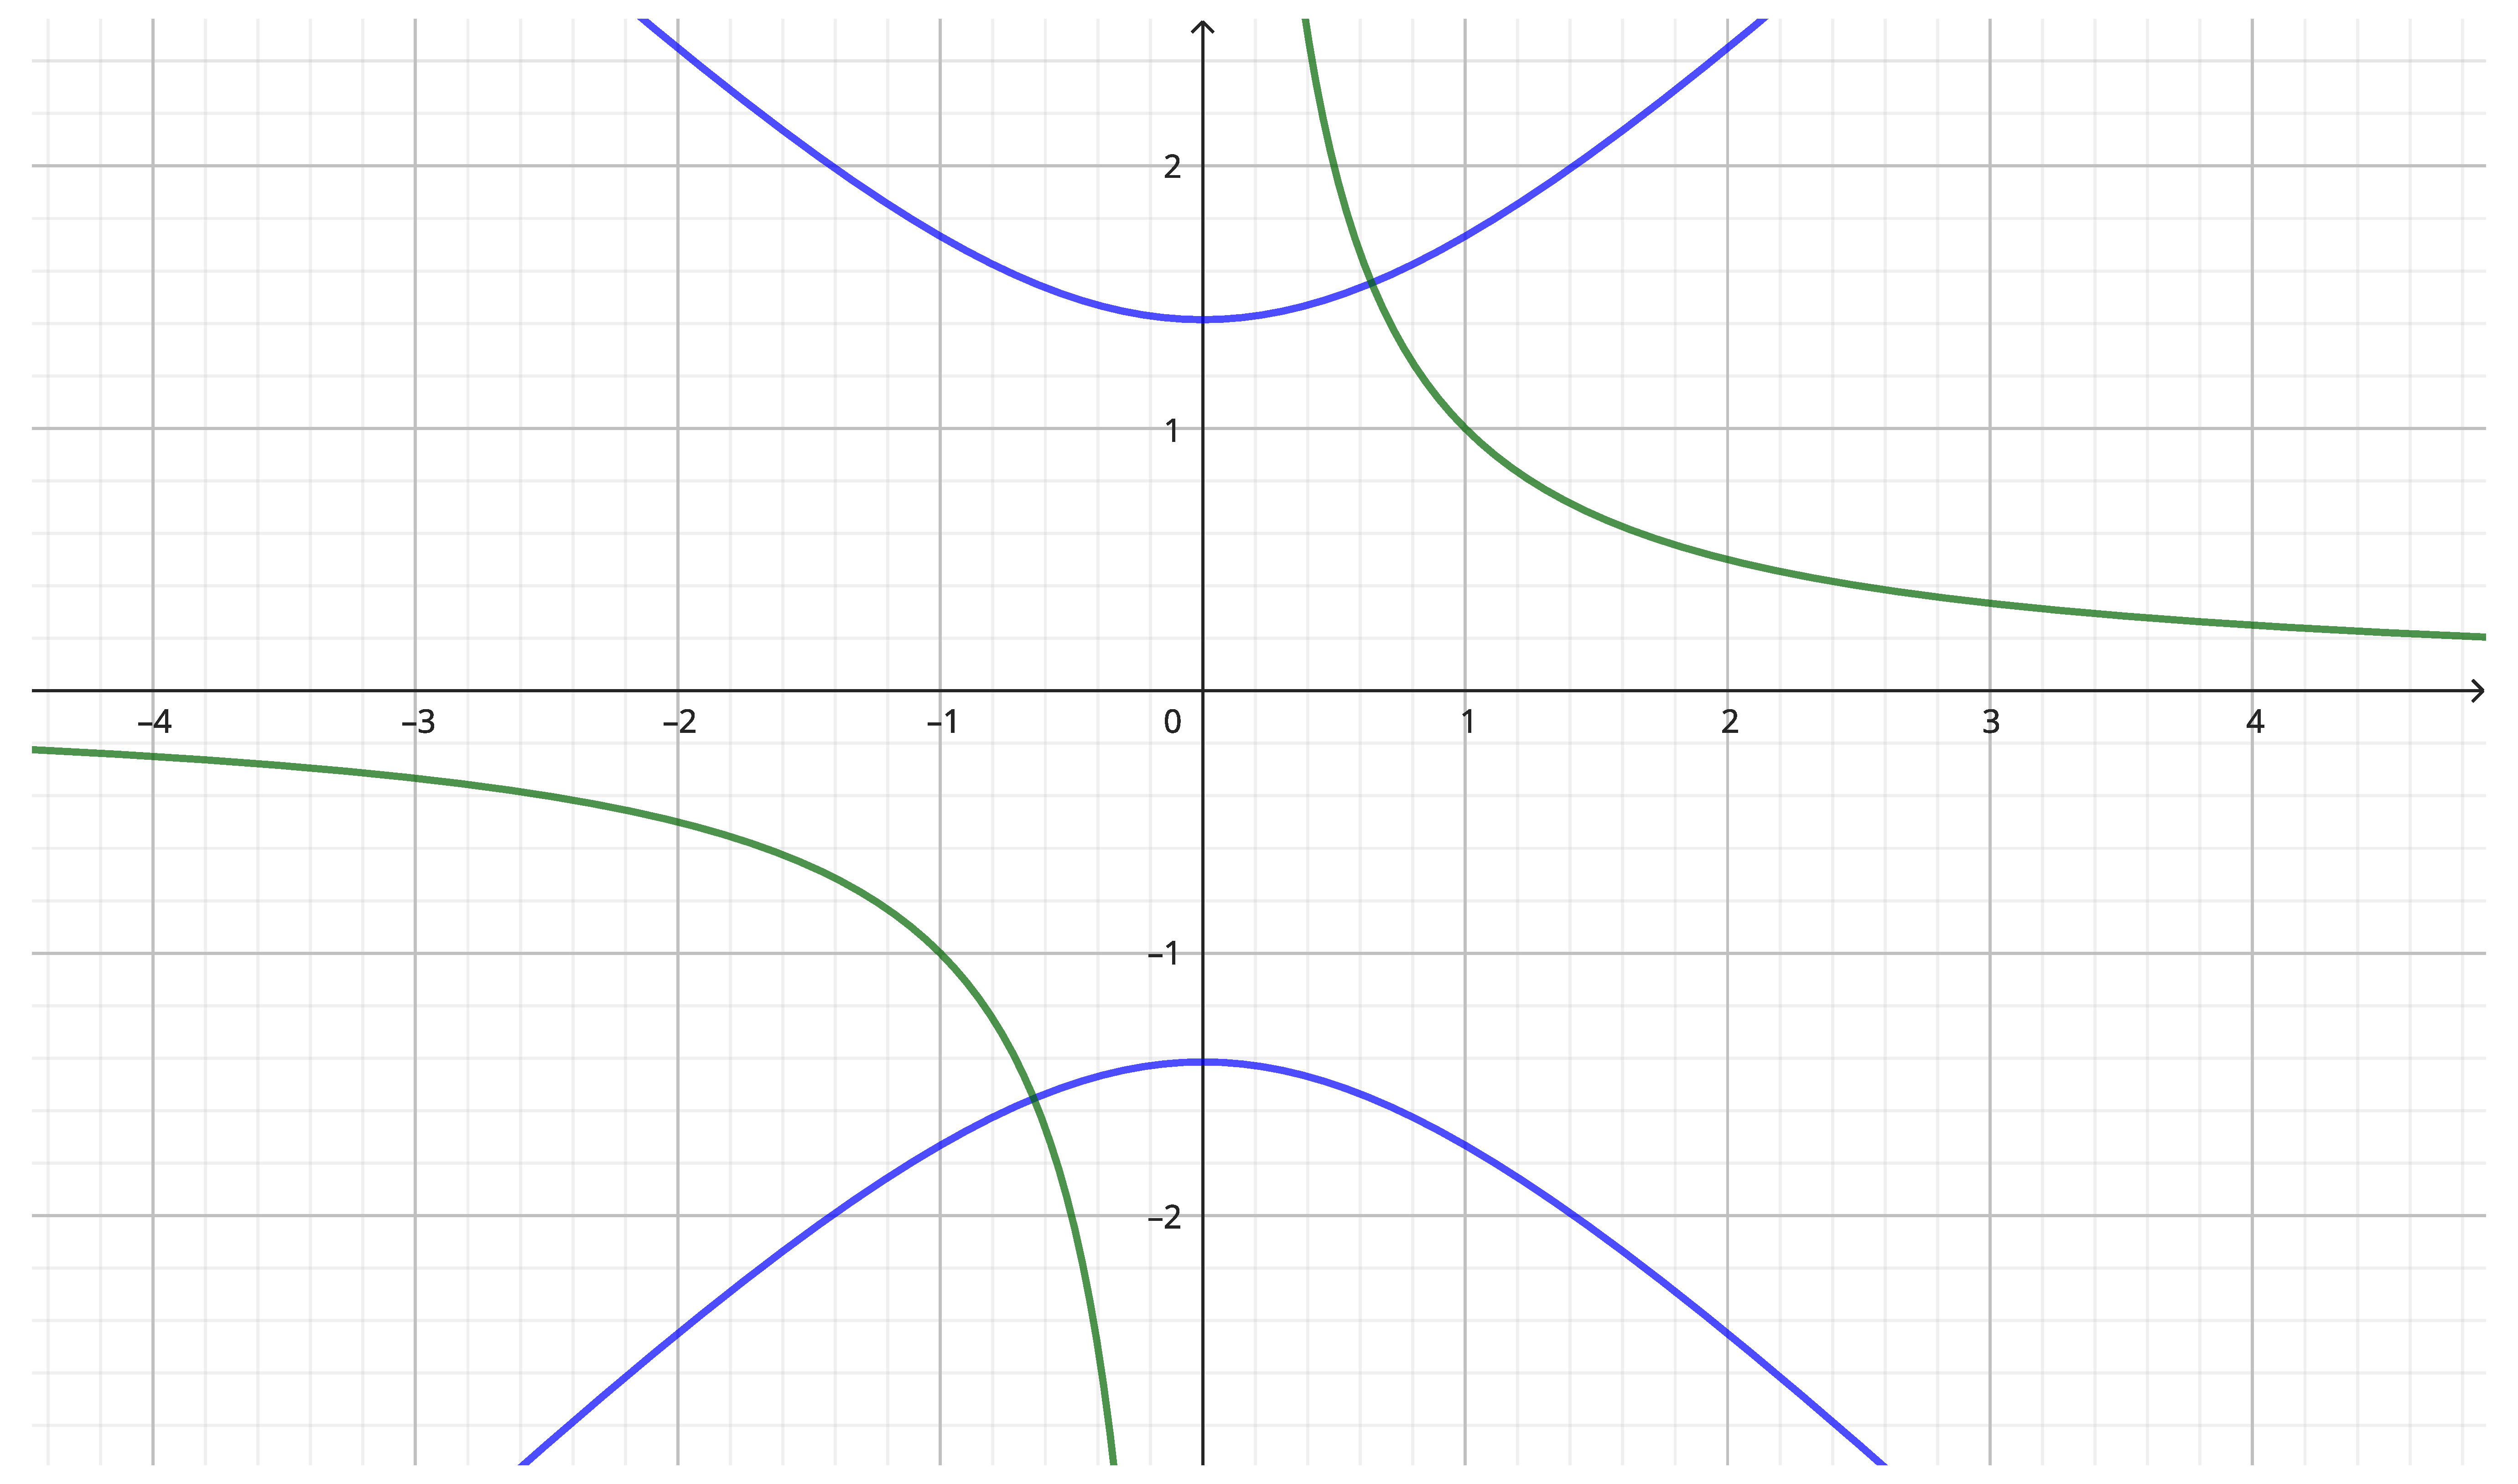
\includegraphics[width=\textwidth]{graph-4.pdf}
            \caption{$xy=1$ (green) and $y^2-x^2=2$ (blue).}
            \label{fig:graph-4}
        \end{figure}
        \begin{gather*}
            \intertext{To transform \eqref{eq:2}, replace $x$ and $y$ with $X$ and $Y$ respectively.}
            XY=1
            \intertext{From \eqref{eq:3}, we get}
            \begin{aligned}
                (x\cos\theta-y\sin\theta)(x\sin\theta+y\cos\theta)&=1\\
                (x^2-y^2)\sin\theta\cos\theta+xy(cos^2\theta-\sin^2\theta)&=1\\
                \frac{1}{2}(x^2-y^2)\sin{2\theta}+xy\cos{2\theta}&=1
            \end{aligned}
            \intertext{When $\theta=\frac{\pi}{4}$,}
            \begin{aligned}
                \frac{1}{2}(x^2-y^2)\sin\frac{\pi}{2}+xy\cos{\frac{\pi}{2}}&=1\\
                \frac{1}{2}(y^2-x^2)&=1
            \end{aligned}
            \intertext{Therefore the transformed function is}
            y^2-x^2=2
        \end{gather*}
        This is an anti-clockwise rotation of the original function $\frac{\pi}{4}$ radians about the origin (Fig. \ref{fig:graph-4}).

    \end{enumerate}

\end{enumerate}

\end{document}
